\section*{Instalasi PIP}

\begin{enumerate}
	\item setelah mendownload file pip. kita bsa masuk ke cmd dengan menekan win+r
	\begin{figure} [h]
	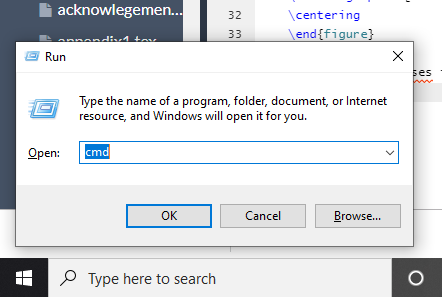
\includegraphics[width=7cm]{section/picpyt/pip/pip1.png}
	\centering
	\end{figure}
	
    \item lalu ketik pip lalu enter
	\begin{figure} [h]
	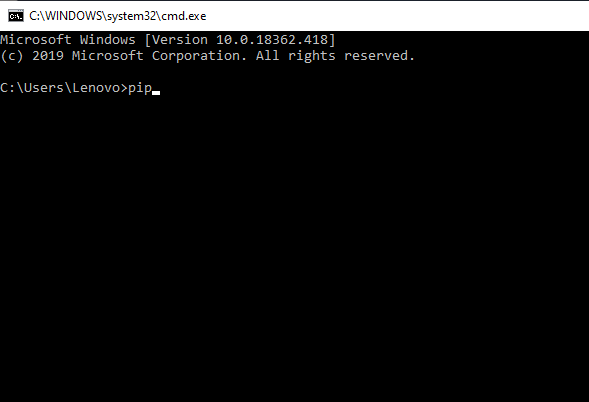
\includegraphics[width=9cm]{section/picpyt/pip/pip2.png}
	\centering
	\end{figure}
	
	\item setelah itu ketik pip install request
	\begin{figure} [h]
	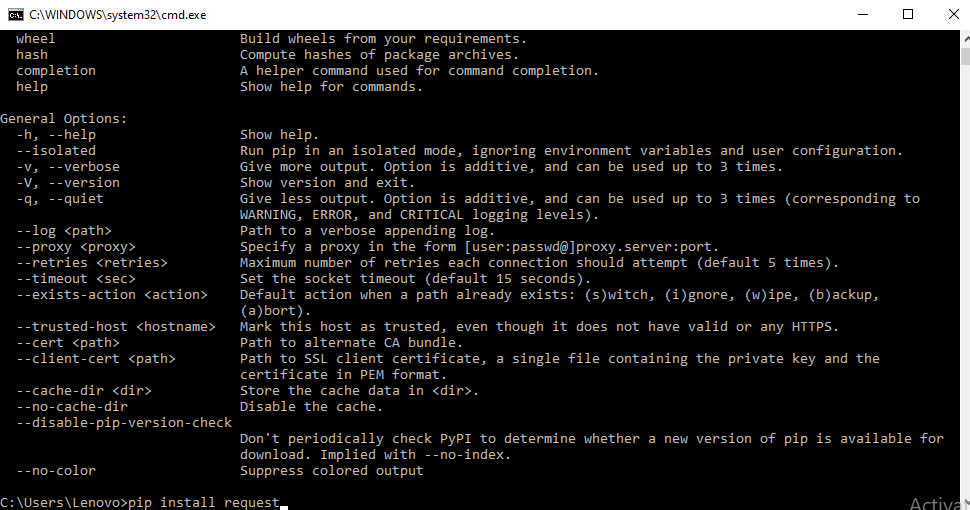
\includegraphics[width=9cm]{section/picpyt/pip/pip4.png}
	\centering
	\end{figure}
	
    \item pip akan mulai menginstall
	
	\item maka pip sudah terinstall
	\begin{figure} [h]
	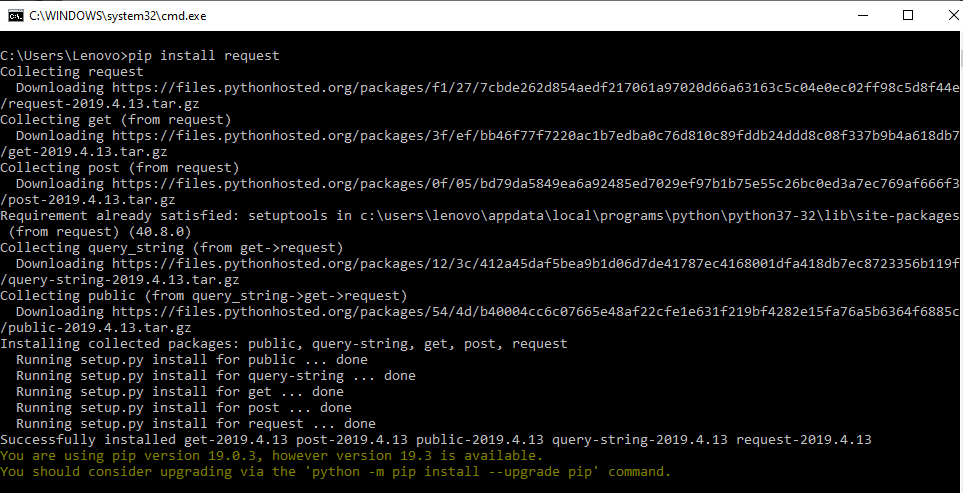
\includegraphics[width=9cm]{section/picpyt/pip/pip5.png}
	\centering
	\end{figure}

\end{enumerate}